% Online supplement: input from main.tex after \appendix
\setcounter{table}{0}
\setcounter{figure}{0}
\renewcommand{\thetable}{A\arabic{table}}
\renewcommand{\thefigure}{A\arabic{figure}}

\section*{Online Supplement}

\subsection*{Part A. Data}

\paragraph{Sources.} Name lists come from the page images of the \textit{TBMM Tutanak Dergisi} published by the Grand National Assembly. For 1943--60, named votes were located in the GNACT page-level text corpus of the minutes (Bo\u{g}azi\c{c}i University; Hugging Face dataset \texttt{boun-tabilab/turkish\_parliamentary\_data}), whose page numbers coincide with those of the official files. A result header (``\ldots\ verilen oyların sonucu'' or ``reylerin neticesi'') followed by a yes tally and at least one other tally identifies a named vote; 1,872 were found for TBMM terms 7--11. Because the corpus's optical character recognition occasionally invents text, it was used only to locate votes and to segment speeches; every list and every quotation used in the article was read from the official page image.

\paragraph{Parsing and reconciliation.} The parser reconstructs columns from word positions, recognizes province and section headings, and checks the resulting lists against the printed tallies (yes, no, abstain, not voting, vacant). The 1945 lists print initials and surnames in capitals (``A.~MENDERES''), so lines carrying an initial were read as names rather than headings; headings garbled by the scans (for example, ``[0]](h ıvatılnrHjanjarl'' for \textit{Oya katılmıyanlar}) were recognized as the next section whose tally is not zero. A vote is used when no list holds more names than its tally, since an overflow indicates that names were filed under the wrong section; names lost to unreadable print leave a deputy's cell empty. Tally misreadings in the text corpus (for example, 17 for 167) were corrected from the page image. Deputies were matched to the Turkish Political Elites Dataset within legislative term and province, by surname and initials (1945) or by full name (1946--80).

\paragraph{Occupations.} The \textit{TBMM Albümü 1920--2010} (Ankara: TBMM, 2010; volumes 1--2, available from the Assembly's open archive) prints for each deputy the place and year of birth, parents, education, languages, occupation, career, and terms served. I parsed 7,355 entries for 1920--80 and matched them to the elites dataset at rates of 97--100 percent in every term. The farmer flag is set when the occupation or career lists \textit{çiftçi}, \textit{çiftçilik}, \textit{ziraatçı}, \textit{çiftlik sahibi}, \textit{arazi sahibi}, \textit{toprak sahibi}, \textit{bağcılık}, \textit{hayvancılık}, or \textit{müstahsil}. Agricultural schooling is coded separately and not counted. The Senate albums are scans without a text layer and were not coded.

\begin{table}[H]
\centering
\begin{threeparttable}
\caption{Roll Calls by Policy Type and Period, and Contested Roll Calls}
\label{tab:A1}
\small
\begin{tabular}{L{7.0cm}rrrrr}
\toprule
Policy type & 1945 & 1946--60 & 1961--80 & Total & Contested, 1946--80 \\
\midrule
\tabinput{tables/ta1_coding.tex}
\bottomrule
\end{tabular}
\begin{tablenotes}\footnotesize
\item \textit{Note:} Assembly roll calls in the harmonized record. 1945 includes all named votes of April 1945--January 1946, which serve as the comparison set for the land law. 1946--60: named votes whose subject is agrarian. 1961--80: National Assembly votes on land, agriculture, and agrarian agencies; the Senate's 245 votes are not included. Contested: the losing side holds at least 5 percent of votes cast; 1945 is excluded because there was no opposition party.
\end{tablenotes}
\end{threeparttable}
\end{table}

\begin{table}[H]
\centering
\begin{threeparttable}
\caption{Coverage and Accuracy of the Record}
\label{tab:A2}
\small
\begin{tabular}{L{3.1cm}L{2.5cm}L{2.5cm}L{3.0cm}L{3.3cm}}
\toprule
 & 1945 & 1946--60 & 1961--80 Assembly & 1961--80 Senate \\
\midrule
Named votes located & 57 & 143 & 322 & 245 \\
Votes used & 54 & 135 & 322 & 245 (not compared) \\
Deputy votes & 19,115 & 60,080 & 137,120 & 44,484 \\
Name format & Initials and surname & Full name & Full name & Full name \\
Lists exact to tally & --- & --- & 72\% of all lists; 85\% within two names & as Assembly \\
Hand verification & Section headings, tallies & Tallies of 3 votes & All 73 land votes exact & 2 manual lists \\
Names matched to deputies & 85\% & 89.5\% & All kept rows (elites dataset) & Senate roster \\
Excluded & 3 lists run into next vote & 5 page mismatches, 3 overflows & --- & --- \\
\bottomrule
\end{tabular}
\begin{tablenotes}\footnotesize
\item \textit{Note:} ``Lists exact to tally'': the number of names in every section equals the printed tally. For 1945 and 1946--60 the criterion for use is that no list exceeds its tally (see text). Page mismatches: the text corpus's page does not exist in the official file, so the list cannot be checked.
\end{tablenotes}
\end{threeparttable}
\end{table}

\subsection*{Part B. The 1945 Land Law}

Figure~\ref{fig:A1} traces the votes of the five deputies who opposed the government's budget on May 29, 1945, across every named vote of April 1945 to January 1946. Their withdrawal begins the day after the budget vote and is general; the land law of June 11 falls within it. In December 1945, Menderes, Köprülü, and Koraltan returned to vote against the 1946 budget. Table~\ref{tab:A3} lists the principal speakers in the debate on the law and the quotations used in the article, with the page of the official minutes on which each was verified.

\begin{figure}[H]
\centering
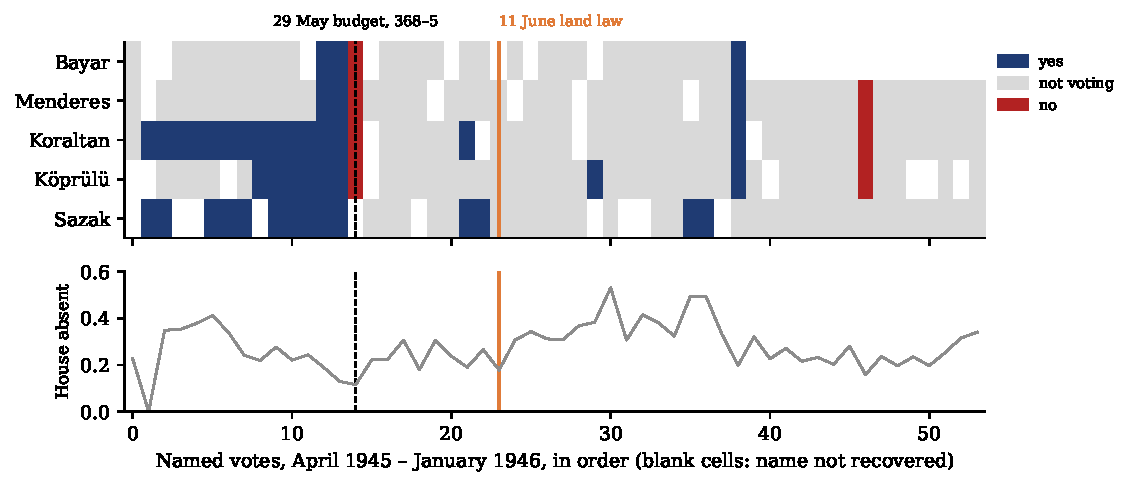
\includegraphics[width=\textwidth]{figA1_1945_withdrawal.pdf}
\caption{The Withdrawal of the Democrat Party Founders, 1945}
\label{fig:A1}
\begin{minipage}{\textwidth}\footnotesize
\textit{Note:} Top: each cell is one named vote, in order. Blank cells: the deputy's name was not recovered from the list. Bottom: share of non-excused deputies not voting. Dashed line: the seven-month budget of May 29, 1945 (368--5). Solid line: the land law of June 11, 1945 (345--0).
\end{minipage}
\end{figure}

\begin{table}[H]
\centering
\caption{The 1945 Land Debate: Principal Speakers and Verified Quotations}
\label{tab:A3}
\footnotesize
\begin{tabular}{L{4.2cm}L{2.1cm}cccrrr}
\toprule
\multicolumn{8}{l}{\textit{Panel A. Sixteen speakers with the most words (sessions 54--58 and 67--72)}} \\
Speaker & Province & Later DP & Farmer & Office & Turns & Words & Property share \\
\midrule
\tabinput{tables/ta3_debate.tex}
\bottomrule
\end{tabular}

\medskip
\begin{tabular}{L{3.1cm}L{2.6cm}L{10.2cm}}
\multicolumn{3}{l}{\textit{Panel B. Quotations (minutes file and page of the official PDF)}} \\
\toprule
Speaker & Date, source & Statement (translated) \\
\midrule
Adnan Menderes & 15.5.1945, 07017055 p.~22 & The bill's farmstead scheme is taken ``almost verbatim'' from the National Socialist hereditary farm law. \\
Refik Koraltan & 14.5.1945, 07017054 p.~30 & ``If the government continues on this path, I cannot trust it.'' \\
Cavit Oral & 4.6.1945, 07018067 p.~32 & ``The provisions of Article 17 recognize no limit in land.'' \\
Adnan Menderes & 4.6.1945, 07018067 p.~41 & Protests that the majority's motion on Article 17 was passed hand to hand for signatures and is adopted without debate; asks not to be counted against the land law. \\
Emin Sazak & 4.6.1945, 07018067 p.~46 & ``If I denied that my tie to land affects my speech and my feelings, I would be lying.'' \\
Emin Sazak & 5.6.1945, 07018068 p.~41 & ``Where are these serfs, these captives?'' \\
Refik Koraltan & 5.6.1945, 07018069 p.~7 & A unanimous vote on the law ``will be a clear answer'' to those who say there is opposition in the Assembly. (He did not vote.) \\
İbrahim Arvas & 13.3.1950, 08025063 p.~20 & At the CHP congress the delegates ``all at once attacked articles 15, 16, 17 and 43.'' \\
Şevket R. Hatipoğlu & 13.3.1950, 08025063 p.~25 & The 1945 law is ``the only legacy of honor I can leave my children.'' \\
Sabit Sağıroğlu & 13.3.1950, 08025063 p.~37 & Sharecropping arrangements ended ``all from the fear of Article 17.'' \\
Yahya Kanbolat (TİP) & 5.5.1966, mm02006092 p.~50 & Untitled land should be registered to its possessor only up to 100 dönüm of dry or 20 of irrigated land. \\
\bottomrule
\end{tabular}
\begin{minipage}{\textwidth}\footnotesize \textit{Note:} Panel A: speaker turns segmented from the minutes and matched to the 1943 roster. Office: speaking for the government or the committee. Property share: property and production terms as a share of property plus redistribution terms in the speaker's turns (a rough lexicon index; later-DP speakers 0.64, others 0.45, permutation $p=.17$). File prefixes: \texttt{tbmm} omitted. In March 1950 the agriculture minister presenting the dilution of the law was Cavit Oral (08025063 pp.~37--39).\end{minipage}

\end{table}

\subsection*{Part C. Tutelage, the Radical Flank, and Robustness}

Figure~\ref{fig:A2} shows the collapse of partisan distance on agrarian roll calls after the military memorandum of March 12, 1971. Figure~\ref{fig:A3} shows the salience of land reform in the minutes. Figure~\ref{fig:A4} reports the ideal-point maps for the remaining terms of the National Assembly. Table~\ref{tab:A4} sets out the comparison of land reform moments, the evidence on the radical flank, and robustness checks.

\begin{figure}[H]
\centering
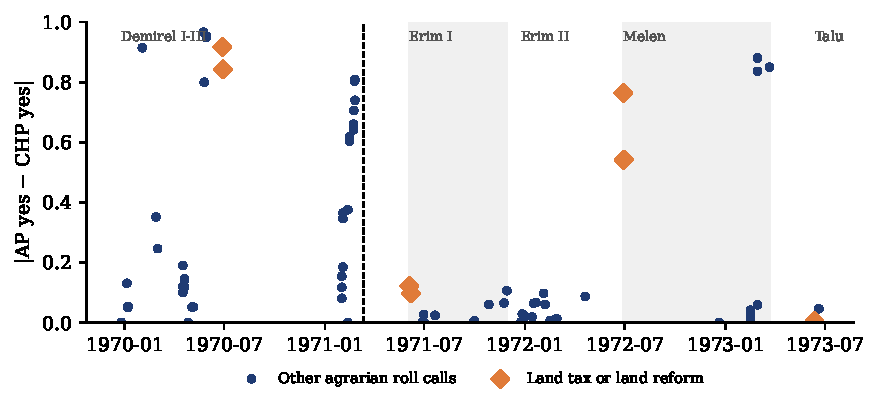
\includegraphics[width=.95\textwidth]{figA2_memorandum.pdf}
\caption{Partisan Distance on Agrarian Roll Calls, 1969--1973}
\label{fig:A2}
\begin{minipage}{\textwidth}\footnotesize
\textit{Note:} Each point is a National Assembly roll call: the absolute difference between the AP and CHP yes shares among votes cast. Bands mark cabinets; dashed line: the memorandum of March 12, 1971. The mean distance fell by 0.38 between the Demirel governments and the post-memorandum period; a placebo in time over 156 break dates in other terms gives $p=.03$.
\end{minipage}
\end{figure}

\begin{figure}[H]
\centering
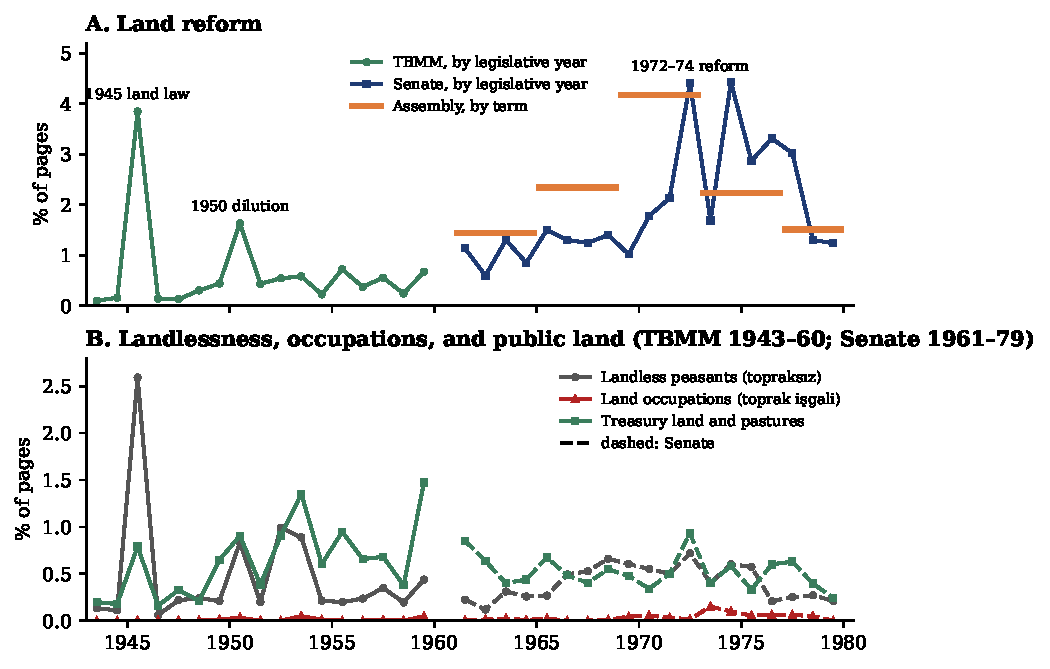
\includegraphics[width=.95\textwidth]{figA3_speech.pdf}
\caption{Land Reform in Parliamentary Speech, 1943--1980}
\label{fig:A3}
\begin{minipage}{\textwidth}\footnotesize
\textit{Note:} Share of pages of the minutes that mention land reform or land distribution (\textit{toprak reformu}, \textit{tarım reformu}, \textit{toprak dağıtımı}, \textit{topraklandırma}), by legislative year (single-chamber TBMM and Senate) and by term (National Assembly). Phrase counts from the text corpus.
\end{minipage}
\end{figure}

\begin{figure}[H]
\centering
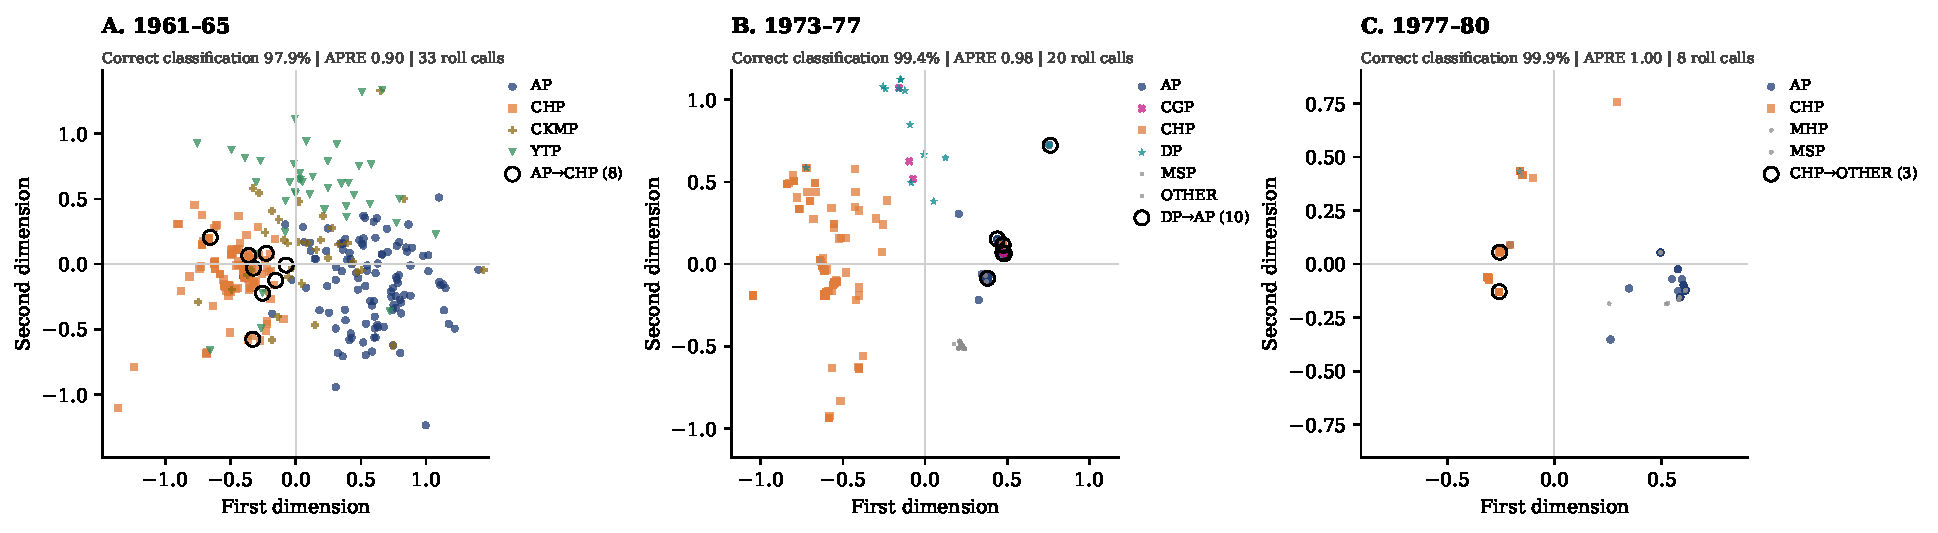
\includegraphics[width=\textwidth]{figA4_split_maps_other.pdf}
\caption{Estimated Positions of Deputies, National Assembly 1961--65, 1973--77, and 1977--80}
\label{fig:A4}
\begin{minipage}{\textwidth}\footnotesize
\textit{Note:} As Figure 1. Circled: deputies whose party at the end of the term differs from that at its start. Fewer agrarian roll calls meet the fitting criterion in 1973--80, so these positions rest on 20 and 8 roll calls.
\end{minipage}
\end{figure}

\begin{table}[H]
\centering
\begin{threeparttable}
\caption{Land Reform Moments, the Radical Flank, and Robustness}
\label{tab:A4}
\footnotesize
\begin{tabular}{L{3.0cm}L{4.1cm}L{3.1cm}L{4.8cm}}
\toprule
\multicolumn{4}{l}{\textit{Panel A. Moments when land reform reached a recorded vote}} \\
Moment & Regime & Recorded result & Opponents' action; outcome \\
\midrule
June 1945 & Single party (CHP) & Land law 345--0 & Voice in debate; founders' general withdrawal; \textbf{passed} \\
March 1950 & Two-party, election due & Dilution 261--15 & Critics rewrite law inside CHP (Oral minister); DP absent; \textbf{diluted} \\
1950--60 & DP majority & Titling and technical amendments only & No extension of distribution reached a vote; \textbf{shelved} \\
February 1965 & Coalitions & Motion 157--167 & AP mobilized (1.65$\times$ attendance), 98\% no; \textbf{defeated} \\
June 1973 & Military-supervised cabinets; TİP closed & Reform law 238--5 & AP 198--1 for; CHP 2 of 101 present; \textbf{passed} \\
\midrule
\multicolumn{4}{l}{\textit{Panel B. The radical flank: Workers' Party of Turkey (TİP), National Assembly 1965--69}} \\
\midrule
Roll calls & 78 & Outcome-pivotal & 0 (TİP's votes never decided an outcome) \\
Quorum-pivotal & 10 (9 passed) & Turnout of TİP & 37\% \\
Mean first dimension & TİP $-1.12$; CHP $-0.65$; AP $+0.34$ & Ceiling amendments (1966) & 100 dönüm dry / 20 irrigated; rejected by show of hands, no recorded vote \\
Quorum rule check & Outcome matches 226-of-450 rule in 289 of 295 roll calls & CHP $\rightarrow$ GP exit & $-0.04$ ($p=.46$) \\
\midrule
\multicolumn{4}{l}{\textit{Panel C. Robustness}} \\
\midrule
Farmer effect by era & 1946--50 $-0.005$ (0.010); 1950--60 $-0.001$ (0.008); 1961--65 $-0.012$ (0.013) & 1965--71 $+0.021$ (0.012); 1971--73 $0.000$ (0.020); 1973--80 $-0.001$ (0.008) & Within party and roll call; contested votes; SE clustered by deputy \\
Government premium, final passage, budgets, and accounts only & 1961--65 0.46; 1965--71 0.64 & 1971--73 0.35; 1973--80 0.84 & All stages: 0.42, 0.59, 0.31, 0.84 \\
1948 exit, alternative split date & January 1948: $+0.10$ & July 1948: $+0.10$ & Departure of the independent group vs.\ founding of the MP \\
1955 exit, all agrarian votes & $-0.16$ ($p<.001$) & Agency budgets: $-0.52$ & Stayers unchanged in both \\
1945 land law, later-DP absence & All 54 votes: DiD $+0.25$, $p=.07$ (votes), $p=.03$ (deputies) & After May 29 only: five founders $+0.21$ ($p=.18$); 14 later-DP $+0.15$ ($p=.15$) & Withdrawal general, not land-specific \\
DID$_M$ placebo & 0.002 [0.000, 0.010] & Turnout placebo 0.03 & Periods without status switches \\
\bottomrule
\end{tabular}
\begin{tablenotes}\footnotesize
\item \textit{Note:} Panel A: see text and Figure 4. Panel B: outcome-pivotal means that reversing TİP's votes would change the result; quorum-pivotal means that TİP's presence or absence decided whether 226 deputies took part. Panel C: estimates as in the main tables with the stated changes.
\end{tablenotes}
\end{threeparttable}
\end{table}
